\documentclass{standalone}
\usepackage{tikz}
\usetikzlibrary{patterns, positioning}
\usepackage[sfdefault]{ClearSans} %% option 'sfdefault' activates Clear Sans as the default text font
\usepackage[T1]{fontenc}

\begin{document}
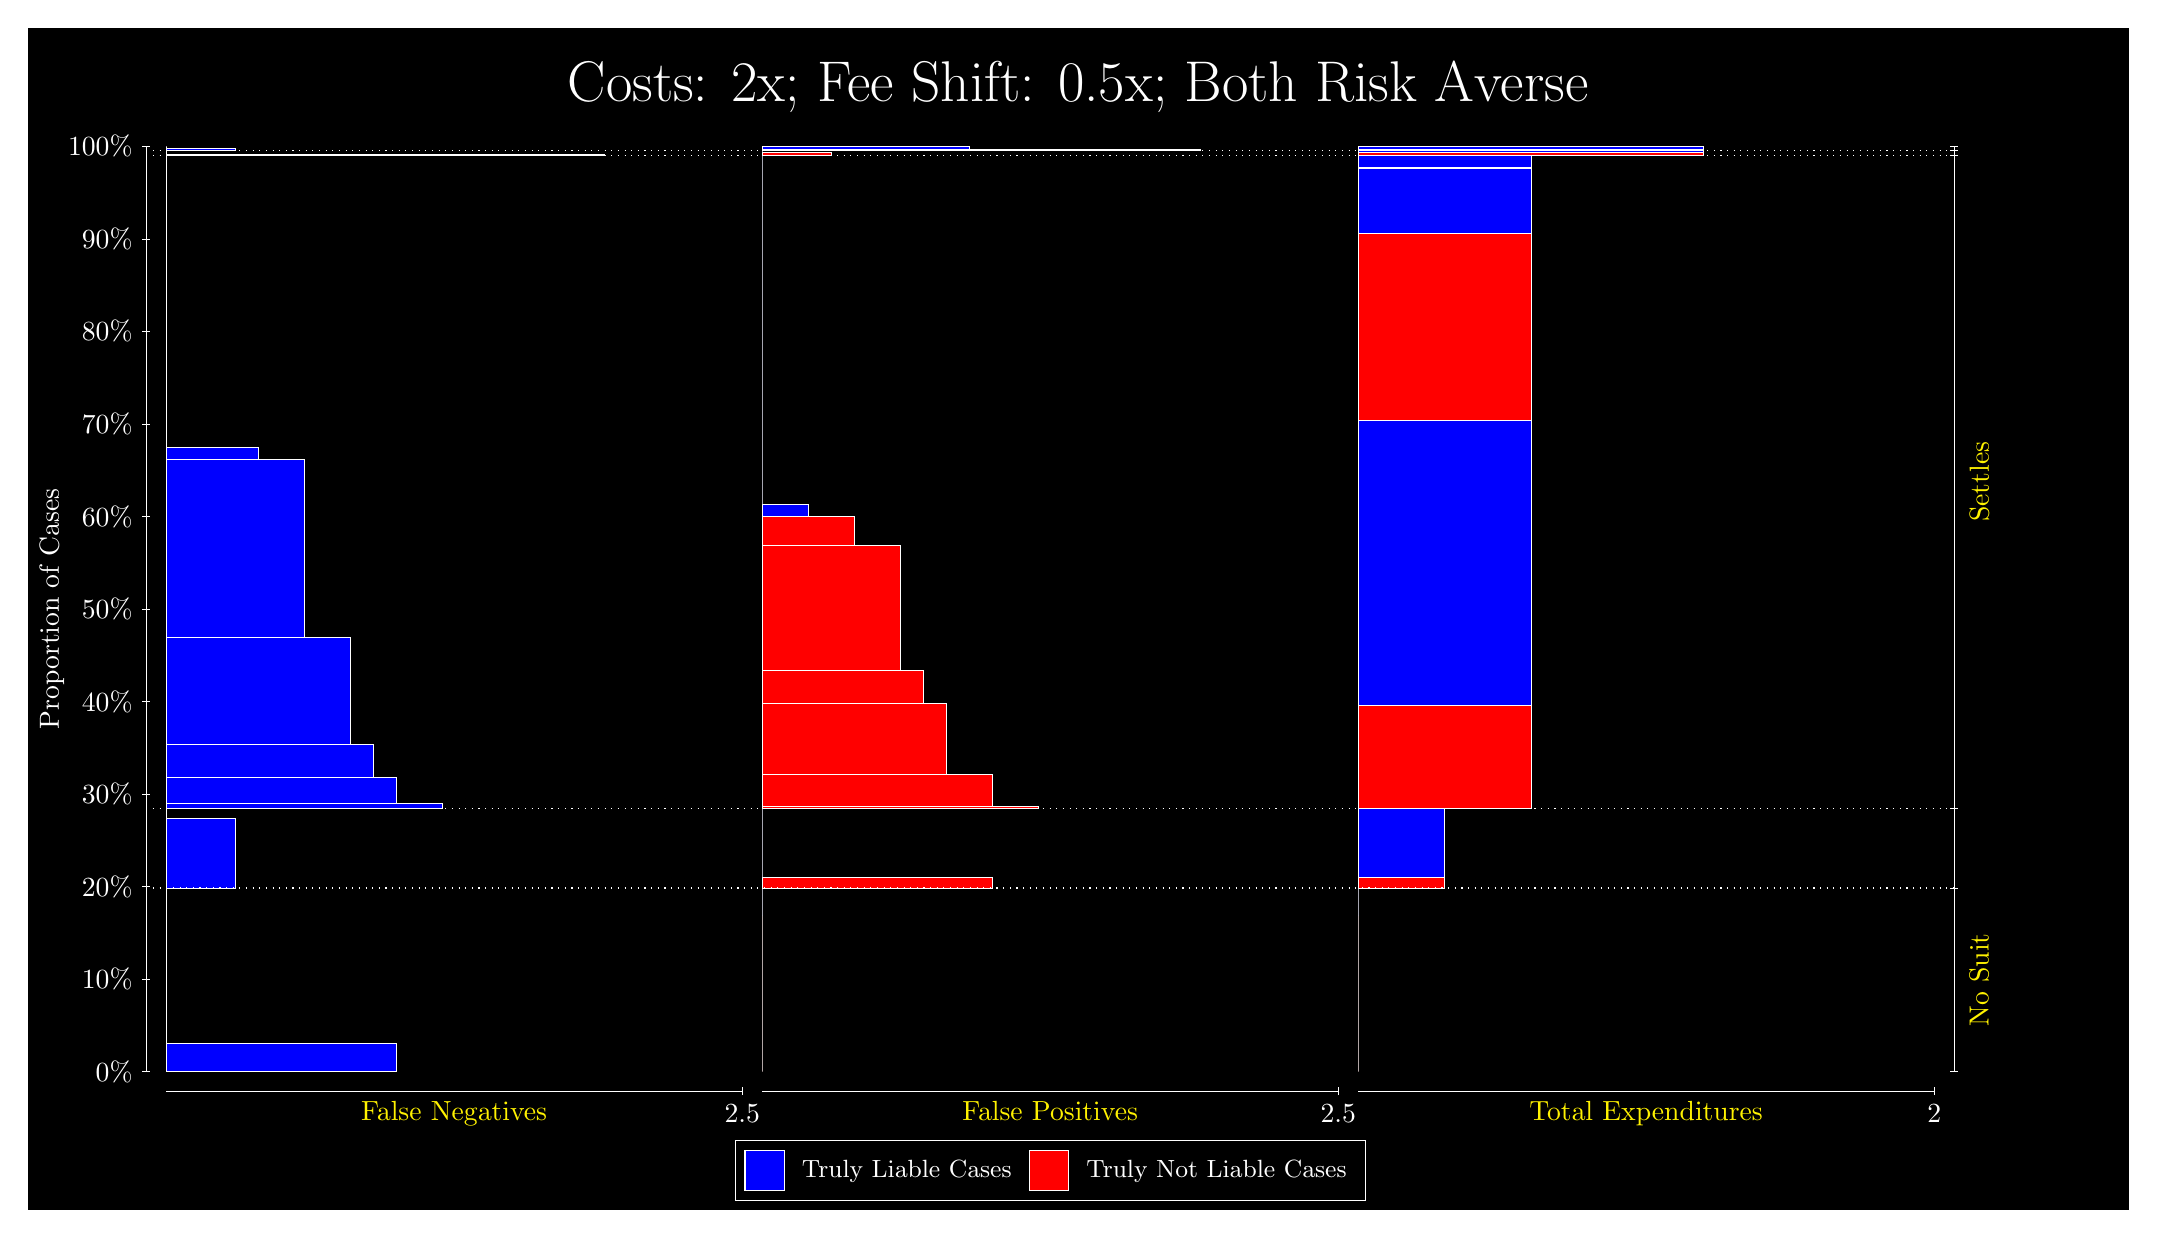
\begin{tikzpicture}
\draw[fill=black] (0,0) rectangle (26.667,15);
\draw[text=white] (0,13.5) rectangle (26.667,15) node[midway] {\huge Costs: 2x; Fee Shift: 0.5x; Both Risk Averse};
\draw[white, very thin] (1.5,1.75) -- (1.5,13.5);
\node[rotate=90, text=white, anchor=center] at (0.3, 7.625) {Proportion of Cases};
\draw[white, very thin] (1.45,1.75) -- (1.55,1.75);
\node[text=white, anchor=east] at (1.45, 1.75) {0\%};
\draw[white, very thin] (1.45,2.925) -- (1.55,2.925);
\node[text=white, anchor=east] at (1.45, 2.925) {10\%};
\draw[white, very thin] (1.45,4.1) -- (1.55,4.1);
\node[text=white, anchor=east] at (1.45, 4.1) {20\%};
\draw[white, very thin] (1.45,5.275) -- (1.55,5.275);
\node[text=white, anchor=east] at (1.45, 5.275) {30\%};
\draw[white, very thin] (1.45,6.45) -- (1.55,6.45);
\node[text=white, anchor=east] at (1.45, 6.45) {40\%};
\draw[white, very thin] (1.45,7.625) -- (1.55,7.625);
\node[text=white, anchor=east] at (1.45, 7.625) {50\%};
\draw[white, very thin] (1.45,8.8) -- (1.55,8.8);
\node[text=white, anchor=east] at (1.45, 8.8) {60\%};
\draw[white, very thin] (1.45,9.975) -- (1.55,9.975);
\node[text=white, anchor=east] at (1.45, 9.975) {70\%};
\draw[white, very thin] (1.45,11.15) -- (1.55,11.15);
\node[text=white, anchor=east] at (1.45, 11.15) {80\%};
\draw[white, very thin] (1.45,12.325) -- (1.55,12.325);
\node[text=white, anchor=east] at (1.45, 12.325) {90\%};
\draw[white, very thin] (1.45,13.5) -- (1.55,13.5);
\node[text=white, anchor=east] at (1.45, 13.5) {100\%};

\draw[white, very thin] (24.457,1.75) -- (24.457,13.5);
\draw[white, very thin] (24.407,1.75) -- (24.507,1.75);
\node[anchor=west] at (24.407, 1.75) {};
\draw[white, very thin] (24.407,4.0803) -- (24.507,4.0803);
\node[anchor=west] at (24.407, 4.0803) {};
\draw[white, very thin] (24.407,5.0947) -- (24.507,5.0947);
\node[anchor=west] at (24.407, 5.0947) {};
\draw[white, very thin] (24.407,13.386) -- (24.507,13.386);
\node[anchor=west] at (24.407, 13.386) {};
\draw[white, very thin] (24.407,13.444) -- (24.507,13.444);
\node[anchor=west] at (24.407, 13.444) {};
\draw[white, very thin] (24.407,13.5) -- (24.507,13.5);
\node[anchor=west] at (24.407, 13.5) {};

\draw[white, very thin, fill=blue] (1.75,1.75) rectangle (4.6775,2.1047);
\draw[white, very thin, fill=red] (1.75,2.1047) rectangle (1.75,4.0803);
\draw[white, very thin, fill=blue] (1.75,4.0803) rectangle (2.6283,4.9615);
\draw[white, very thin, fill=red] (1.75,4.9615) rectangle (1.75,5.0947);
\draw[white, very thin, fill=blue] (1.75,5.0947) rectangle (5.2631,5.152);
\draw[white, very thin, fill=blue] (1.75,5.152) rectangle (4.6775,5.4914);
\draw[white, very thin, fill=blue] (1.75,5.4914) rectangle (4.3848,5.9103);
\draw[white, very thin, fill=blue] (1.75,5.9103) rectangle (4.092,7.264);
\draw[white, very thin, fill=blue] (1.75,7.264) rectangle (3.5065,9.5301);
\draw[white, very thin, fill=blue] (1.75,9.5301) rectangle (2.921,9.6778);
\draw[white, very thin, fill=red] (1.75,9.6778) rectangle (1.75,13.386);
\draw[white, very thin, fill=blue] (1.75,13.386) rectangle (7.3123,13.405);
\draw[white, very thin, fill=red] (1.75,13.405) rectangle (1.75,13.444);
\draw[white, very thin, fill=blue] (1.75,13.444) rectangle (2.6283,13.481);
\draw[white, very thin, fill=red] (1.75,13.481) rectangle (1.75,13.5);
\draw[white, very thin, fill=red] (9.3189,1.75) rectangle (9.3189,3.7255);
\draw[white, very thin, fill=blue] (9.3189,3.7255) rectangle (9.3189,4.0803);
\draw[white, very thin, fill=red] (9.3189,4.0803) rectangle (12.246,4.2134);
\draw[white, very thin, fill=blue] (9.3189,4.2134) rectangle (9.3189,5.0947);
\draw[white, very thin, fill=red] (9.3189,5.0947) rectangle (12.832,5.1164);
\draw[white, very thin, fill=red] (9.3189,5.1164) rectangle (12.246,5.5302);
\draw[white, very thin, fill=red] (9.3189,5.5302) rectangle (11.661,6.4292);
\draw[white, very thin, fill=red] (9.3189,6.4292) rectangle (11.368,6.8456);
\draw[white, very thin, fill=red] (9.3189,6.8456) rectangle (11.075,8.4286);
\draw[white, very thin, fill=red] (9.3189,8.4286) rectangle (10.49,8.8031);
\draw[white, very thin, fill=blue] (9.3189,8.8031) rectangle (9.9044,8.9508);
\draw[white, very thin, fill=blue] (9.3189,8.9508) rectangle (9.3189,13.386);
\draw[white, very thin, fill=red] (9.3189,13.386) rectangle (10.197,13.425);
\draw[white, very thin, fill=blue] (9.3189,13.425) rectangle (9.3189,13.444);
\draw[white, very thin, fill=red] (9.3189,13.444) rectangle (14.881,13.463);
\draw[white, very thin, fill=blue] (9.3189,13.463) rectangle (11.954,13.5);
\draw[white, very thin, fill=red] (16.888,1.75) rectangle (16.888,3.7255);
\draw[white, very thin, fill=blue] (16.888,3.7255) rectangle (16.888,4.0803);
\draw[white, very thin, fill=red] (16.888,4.0803) rectangle (17.986,4.2134);
\draw[white, very thin, fill=blue] (16.888,4.2134) rectangle (17.986,5.0947);
\draw[white, very thin, fill=red] (16.888,5.0947) rectangle (19.083,6.4075);
\draw[white, very thin, fill=blue] (16.888,6.4075) rectangle (19.083,10.027);
\draw[white, very thin, fill=red] (16.888,10.027) rectangle (19.083,12.401);
\draw[white, very thin, fill=blue] (16.888,12.401) rectangle (19.083,13.217);
\draw[white, very thin, fill=red] (16.888,13.217) rectangle (19.083,13.239);
\draw[white, very thin, fill=blue] (16.888,13.239) rectangle (19.083,13.386);
\draw[white, very thin, fill=red] (16.888,13.386) rectangle (21.279,13.425);
\draw[white, very thin, fill=blue] (16.888,13.425) rectangle (21.279,13.444);
\draw[white, very thin, fill=red] (16.888,13.444) rectangle (21.279,13.463);
\draw[white, very thin, fill=blue] (16.888,13.463) rectangle (21.279,13.5);
\draw[white, dotted] (1.5,4.0803) -- (24.457,4.0803);
\draw[white, dotted] (1.5,5.0947) -- (24.457,5.0947);
\draw[white, dotted] (1.5,13.386) -- (24.457,13.386);
\draw[white, dotted] (1.5,13.444) -- (24.457,13.444);
\draw[white, very thin] (1.75,1.5) -- (9.0689,1.5);
\node[text=yellow, anchor=north] at (5.4094, 1.5) {False Negatives};
\draw[white, very thin] (9.0689,1.45) -- (9.0689,1.55);
\node[text=white, anchor=north] at (9.0689, 1.45) {2.5};

\draw[white, very thin] (9.3189,1.5) -- (16.638,1.5);
\node[text=yellow, anchor=north] at (12.978, 1.5) {False Positives};
\draw[white, very thin] (16.638,1.45) -- (16.638,1.55);
\node[text=white, anchor=north] at (16.638, 1.45) {2.5};

\draw[white, very thin] (16.888,1.5) -- (24.207,1.5);
\node[text=yellow, anchor=north] at (20.547, 1.5) {Total Expenditures};
\draw[white, very thin] (24.207,1.45) -- (24.207,1.55);
\node[text=white, anchor=north] at (24.207, 1.45) {2};

\node[text=yellow, centered, rotate=90] at (24.777, 2.9151) {No Suit};

\node[text=yellow, centered, rotate=90] at (24.777, 9.2405) {Settles};



\draw (12.978300999999998,1.5) node[draw=none] (baseCoordinate) {};
\begin{scope}[align=center]
        \matrix[scale=0.5, draw=white, below=0.5cm of baseCoordinate, nodes={draw}, column sep=0.1cm]{
            \node[rectangle, draw, minimum width=0.5cm, minimum height=0.5cm, fill=blue] {}; &
            \node[draw=none, font=\small, text=white] (B) {Truly Liable Cases}; &
            \node[rectangle, draw, minimum width=0.5cm, minimum height=0.5cm, fill=red] {}; &
            \node[draw=none, font=\small, text=white] (B) {Truly Not Liable Cases}; \\
            };
\end{scope}

\end{tikzpicture}
\end{document}